\chapter{Opdracht 1: Projectopzet en analyse}

\section{Stap 1: Zet het project op}
Gebruik voor het project \textit{Java}, versie 11 of hoger.

Verder gebruiken we \textit{Maven}, een tool waarmee je Java-projecten kan opzetten
en gemakkelijk third-party dependencies, zoals frameworks en libraries, kunt 
gebruiken in je project. Zie hiervoor de pom.xml. Maven hoef je niet per se te 
installeren. We kunnen hiervoor onze Integrated Development Environment (IDE) gebruiken.
Ook is er een wrapper (mvnw) opgenomen in het project mocht je de commandline willen gebruiken (aanrader!). 

\subsection{Clone het project}
Clone het GitHub-project via de link die op Canvas wordt aangeboden.
We gebruik hiervoor private repositories binnen GitHub Education.
Zorg dat je een clone krijgt binnen GitHub om je werk in te leveren 
en op je machine om te werken. Open de root-directory van het project
via IntelliJ.

\subsection{Starten met Docker}
Heb je het project op je machine staan? Open het in je IDE (bij voorkeur IntelliJ).

Je kan het project op twee manieren opzetten: met Docker of zonder Docker. 
Zie ook de README.md van het project. 

Het wordt aangeraden om Docker en docker-compose te gebruiken om het project op te starten.
Docker zorgt ervoor dat de technische afhankelijkheden niet apart geïnstalleerd hoeven te worden,
maar herbruikbaar in het project zelf kunnen worden opgenomen.
Docker wordt daarom veel gebruikt in de praktijk om de infrastructuur gelijksoortig te houden 
of je nu op development-, test- of productie-omgeving aan het werk bent.

In het geval van dit project gaat het om een voorgeconfigureerde PostgreSQL-database.

\subsubsection{Installeer Docker}
Download en installeer Docker desktop via de 
\href{https://www.docker.com/products/docker-desktop}{Docker download pagina}.
Volg de instructies op genoemd op de site.
Vraag studenten en docenten om hulp als je er niet uit komt.

\subsubsection{Opstarten met docker-compose}
Als Docker geïnstalleerd is, kan je de database opstarten met docker-compose.
Navigeer in de commandline naar de project directory (je kunt in je IDE meestal ook een terminal window openen).
In de project directory kan je \texttt{docker-compose up} draaien vanaf de commandline. 
De eerste keer duurt dit even: de container voor PostgreSQL wordt gedownload, geconfigureerd,
gebouwd als image en vervolgens wordt de image opgestart.
De volgende keer dat je docker-compose runt wordt alleen de voorgeconfigureerde image opgestart.

Als je de database op de achtergrond wil draaien (in plaats van dat hij actief in je commandline blijft),
kan je ook \texttt{docker-compose start} gebruiken in plaats van \texttt{docker-compose up}.

Gaat er iets mis met \texttt{docker-compose} en wil je de container image opnieuw bouwen,
dan kan je \texttt{docker-compose up --build -V} gebruiken.

Hoe dit precies werkt hoef je voor deze cursus niet te weten,
maar ben je hierin geïnteresseerd, kijk dan eens naar de \texttt{docker-compose.yml}
en in \texttt{development/db} binnen het project. Hier staat alles in gedefinieerd.
Zo wordt er een algemene admin-gebruiker voor PostgreSQL met als username en password 
\texttt{admin} en \texttt{admin} aangemaakt. Ook worden er automatisch username, password en database 
aangemaakt onder de naam \texttt{bep2-huland-casino}.

De standaardpoort van PostgreSQL is \texttt{5321}. Wij herschrijven deze poort in docker-compose.yml
naar \texttt{15432} om conflicten te voorkomen met een bestaande PostgreSQL instantie. 
De connectiedetails worden beschreven in de projectconfiguratie onder src/main/resources/application.properties:

\begin{minted}{ini}
spring.datasource.url=jdbc:postgresql://localhost:15432/bep2-huland-casino
spring.datasource.username=bep2-huland-casino
spring.datasource.password=bep2-huland-casino
\end{minted}

Zie hieronder meer over hoe je moet verbinden met PostgreSQL.

\subsubsection{Problemen oplossen met Docker / PostgreSQL}
Check altijd of Docker Desktop draait en of onze PostgreSQL-image wel is opgestart!

Als data niet lijkt te worden opgeslagen in Docker, zorg dan dat Docker een `volume' kent om 
naar weg te schrijven. Voeg deze directory of de parent directory toe via de Docker user interface 
onder \texttt{Settings > Resources > File Sharing}.

Als je niet met de database lijkt te kunnen verbinden, check dan of Docker 
wel bij het (virtuele) netwerk van de host kan.

\subsection{Starten zonder Docker}
Hoewel Docker wordt aangeraden, kan het voorkomen dat dit op jouw systeem 
om wat voor een reden dan ook niet lukt. Dan moeten we PostgreSQL handmatig instellen.
Daarvoor moeten we een aantal zaken handmatig installeren en configureren in het project.

\subsubsection{PostgreSQL installeren}
Zorg dat PostgreSQL geïnstalleerd is. Dit moet je ook voor de cursus Data & Persistency doen.
Je kan ook de instructies voor die cursus erbij pakken!
Zie: \href{https://www.postgresql.org/download/}{Postgres website}.

Dit is een database die je gebruikt voor de ontwikkeling van webapplicaties met persistentie.
Zorg dat je de hoofddatabase en de admin-inloggegevens onthoudt of bewaart.
Ben je dit vergeten, dan kan je het best PostgreSQL opnieuw installeren.

\subsubsection{Verbinden met de database}
Zorg dat je een tool hebt om handmatig te verbinden met de database.
Hiervoor kan je je \textit{IntelliJ} gebruiken of een tool als \textit{pgAdmin}.
Om via IntelliJ te verbinden, kan je de instructies uitvoeren die te vinden zijn op:
\href{https://www.jetbrains.com/help/idea/connecting-to-a-database.html#connect-to-postgresql-database}{Helppagina Jetbrains}.
De instructies zijn vergelijkbaar voor DataGrip.

Voor \textit{pgAdmin}, zie: \href{https://www.pgadmin.org/}{Website pgAdmin}.

De volgende gegevens heb je nodig voor het verbinden met de hoofddatabase:
\begin{itemize}
    \item \textbf{Host}: \texttt{localhost}
    \item \textbf{Port}: \texttt{5432} (met Docker: \texttt{15432})
    \item \textbf{Database}: \texttt{<admin database>} (met Docker: \texttt{postgres})
    \item \textbf{Username}: \texttt{<admin user>} (met Docker: \texttt{admin})
    \item \textbf{Username}: \texttt{<admin password>} (met Docker: \texttt{admin})
\end{itemize}

\subsubsection{Database en gebruikers instellen}
Als we geen Docker hebben gebruikt, moeten we zorgen dat de database, username en password voor \texttt{bep2-huland-casino}
worden aangemaakt. Hiervoor kan je de volgende queries uitvoeren.

De user (en password) maak je aan met de volgende SQL-query (gebruik een raw query in je database-tool):
\begin{minted}{sql}
CREATE USER "bep2-huland-casino" WITH CREATEDB PASSWORD 'bep-huland-casino';
\end{minted}

De database maak je als volgt aan met de juiste gebruiker (gebruik een raw query in je database-tool): 
\begin{minted}{sql}
CREATE DATABASE "bep2-huland-casino" OWNER "bep2-huland-casino";
\end{minted}

\subsubsection{Projectinstellingen veranderen}
De standaardpoort van PostgreSQL is \texttt{5321}. 
Ons project staat ingesteld om te verbinden met poort \texttt{15321}, omdat we 
dat met Docker doen om niet met andere PostgreSQL-instanties in de knoop te komen.

We kunnen aanpassen hoe onze applicatie met de applicatie verbindt via 
de configuratie in src/main/resources/application.properties.
Zorg dat deze er als volgt uitziet:
\begin{minted}{ini}
spring.datasource.url=jdbc:postgresql://localhost:5432/bep2-huland-casino
spring.datasource.username=bep2-huland-casino
spring.datasource.password=bep2-huland-casino
\end{minted}

Heb je iets veranderd en werkt het? 
Commit je wijzigingen met een duidelijke naam, 
bijvoorbeeld: "Customize database configuration". 
Push de wijzigingen naar je remote GitHub repository.

\subsection{De applicatie starten}
Als onze database draait kunnen we onze applicatie starten.
Dit kunnen we doen door in onze IDE op de play-knop te drukken naast de main-method 
van de klasse CasinoApplication. Of het Maven-commando \texttt{spring-boot:start}.
Dit commando kan je in de IDE uitvoeren (Maven-paneel rechts of via het menu \texttt{View > Tool Windows > Maven}). 
Ook kan je de commandline gebruiken: \texttt{mvnw spring-boot:start}.

Als het goed is, zie je nu in de commandline allerlei log-berichten. De laatste regels 
zouden moeten gaan over dat de applicatie te bereiken is op poort \texttt{8080}.
Zie je dit niet en in plaats daarvan een lange foutmelding. Scroll dan omhoog (of omlaag)
naar de plek waar je meer informatie kan vinden over deze fout. Probeer dit te googelen 
om er meer over te weten te komen. 

Twee veelvoorkomende fouten:
\begin{itemize}
    \item De database is onbereikbaar: zorg dat je bovenstaande instructies hebt gevolgd om de database (met of zonder Docker)
    draaiende te krijgen.
    \item De poort 8080 is al in gebruik: er draait al een web-applicatie op poort 8080. 
    Sluit deze applicatie af of stel een andere poort in in de application.properties.
\end{itemize}

Kan je de fout niet oplossen? Trek dan even aan de bel bel je docent of medestudenten!

\subsection{Web requests uittesten met Postman}
We gebruiken Postman als HTTP-client. Een HTTP-client is een programma dat 
HTTP-requests kan versturen en HTTP-responses kan ontvangen.
Normaliter doet je web browser dit (vaak met behulp van wat JavaScript).

Dit project wordt geleverd met een Postman-collection,
hierin zitten al wat standaard requests en wat scripts om het inloggen
en ingelogd blijven via Postman gemakkelijker te maken. Dit is namelijk 
geen expliciet onderdeel van de cursus.

\subsubsection{Installeer Postman}
Ga naar \href{https://www.postman.com/downloads/}{de Postman website} 
en installeer de Postman client.

\subsubsection{Importeer de Postman-collection}
We hebben voor dit project al een standaardcollectie opgenomen met 
de requests die we kunnen uitvoeren voor inloggen, registratie en 
chips use cases.

Laten we die acties gaan uitvoeren. Importeer de collection
\\ "bep2-huland-casino.postman\_collection.json" die te 
vinden is in het project.

Het handige aan deze collectie is dat hij voor elke actie ook 
de JWT token meestuurt! Anders zou je dit elke keer met de hand 
mee moeten sturen in de request headers.

\subsubsection{Voer requests uit}
Je ziet dat we al een aantal requests klaar hebben staan.
Het idee is dat we tijdens dit project zelf ook een aantal requests
gaan toevoegen om Blackjack te kunnen spelen!

Laten we een nieuwe gebruiker aanmaken, de inloggen, zijn chips bekijken en nieuwe chips storten.
\begin{enumerate}
    \item \textbf{auth, POST register}: registreer een gebruiker.
    Je kan de waarden aanpassen door naar "Body" te gaan als je wilt.
    \item \textbf{auth, POST login}: login als de gebruiker die je zojuist
    hebt aangemaakt. Pas de waarden aan in de request body indien nodig.
    \item \textbf{chips, GET show balance}: laat de chips zien van de huidige 
    ingelogde gebruiker. Hiervoor wordt de meegestuurde token gebruikt
    (dit hebben wij ingesteld in de Postman collectie)
    \item \textbf{chips, POST deposit}: stort chips.
    In de body kan je de amount aanpassen.
\end{enumerate}

Lukt er iets niet? Kijk of je de fout kunt achterhalen door 
naar de logs te kijken in je IDE. Bespreek het met medestudenten 
en docenten als je er niet uit komt of iets niet begrijpt.

Heb je iets veranderd om het werkend te krijgen? Sla je werk op. 
Commit je wijzigingen met een duidelijke naam, 
bijvoorbeeld: "Improve URLs in Postman collection". 
Push de wijzigingen naar je remote GitHub repository.

Misschien is het ook iets waar de docenten of andere studenten 
wat aan hebben!

\newpage
\section{Stap 2: Bereid je voor}
Heb je de database opgezet en de functionaliteit getest? Keurig!
Laten we nu eens kijken wat er van ons verwacht wordt met dit project.

\subsection{Neem de opdrachtbeschrijving door}
Neem de opdrachtbeschrijving en de opdracht op Canvas door. 
Kan je (voor jezelf) antwoord geven op de volgende vragen?

\begin{enumerate}
    \item Wat moeten we precies maken?
    \item Waarom is er gekozen voor een web-applicatie?
    \item Hoe werkt blackjack ongeveer?
    \item Wat ga je ongeveer leren met deze cursus?
    \item Waar word je op beoordeeld?
    \item Waar krijg je de meeste punten voor?
    \item Wat moet je doen voor een voldoende?
\end{enumerate}

In het verleden is gebleken dat veel studenten erg laat beginnen 
en daarmee in de knoop komen met andere cursussen. Probeer dat te 
voorkomen door regelmatig je werk in te leveren, zodat je continu feedback 
kunt krijgen. Het is dus handig om voor jezelf een planning te maken.
De opdracht is om die reden opgedeeld in 6 stappen die ongeveer gelijk lopen 
met de inhoudelijke invulling van de werkcolleges.
Maak je je op enig punt tijdens de cursus zorgen over de planning,
geef het aan!

\subsection{Extra informatie: de projectstructuur}
Studenten hebben aangegeven meer informatie te willen ontvangen over hoe het 
systeem is opgezet. Daar is dit onderdeel voor bedoeld. Het is niet 
erg als je nog niet alles helemaal begrijpt of dat je niet overtuigd 
bent van deze opzet. Het gaat erom dat je in hoofdlijnen doorhebt 
waar wat te vinden is. Tijdens deze cursus gaan we er dieper op in.

Laten we eens kijken naar hoe het project is opgezet.
Onder src/main/java zien we onze packagestructuur.
Met behulp van packages kunnen we ons systeem op een logische manier 
ordenen. Dit is een belangrijke stap in het bereiken van 
\textit{separation of concerns, high cohesion en loose coupling}!

Structurele kwaliteit ziet immers op de onderhoudbaarheid
van een softwareproject. Een softwareproject heeft in algemene zin 
een goede structuur als deze is opgedeeld in kleine,
opzichzelf staande modules die intern veel samenhang 
en met elkaar beperkt koppeling vertonen.

\newpage
\subsubsection{Packagestructuur in Java}
In Java kunnen we modules groeperen door gebruik te maken van 
\emph{packages} (in C\# en andere talen met \emph{namespaces}).
De naam van een Java-package lijkt op een soort omgekeerd webadres
en komt overeen met de onderliggende mappenstructuur.
Het is gebruikelijk om in Java-packages eerst te beginnen met de organisatienaam,
bijvoorbeeld \texttt{nl.hu.bep2}, en vervolgens de projectnaam \texttt{casino}.
Dan kunnen we het project opdelen in componenten, zoals in het casino-project: 
\begin{itemize}
\item \texttt{nl.hu.bep2.casino.chips}
\item \texttt{nl.hu.bep2.casino.security}
\item \texttt{nl.hu.bep2.casino.blackjack}
\end{itemize}

Binnen elk component kan met packages 
onderscheid gemaakt worden naar het soort logica volgens een gelaagde aanpak. 
Dat leidt bij het casino-project tot de volgende 
mappen- en packagestructuur onder \texttt{src/main/java}:

\dirtree{%
    .1 nl.hu.bep2.casino.
        .2 chips.
            .3 presentation.
                .4 controller.
                .4 dto.
            .3 application.
            .3 domain.
                .4 exception.
            .3 data.
        .2 security.
            .3 presentation.
                .4 controller.
                .4 dto.
                .4 filter.
            .3 application.
            .3 domain.
            .3 data.
        .2 blackjack.
            .3 (...).
}

Het project is dus eerst opgedeeld in verschillende componenten en vervolgens in 
lagen. In lagen kunnen we zaken weer groeperen in deelsystemen. Deze componenten 
en lagen kunnen we weergeven als packages, zie Figuur~\ref{fig:uml-casino-physical-layers}.

\begin{figure}[H]
    \centering
    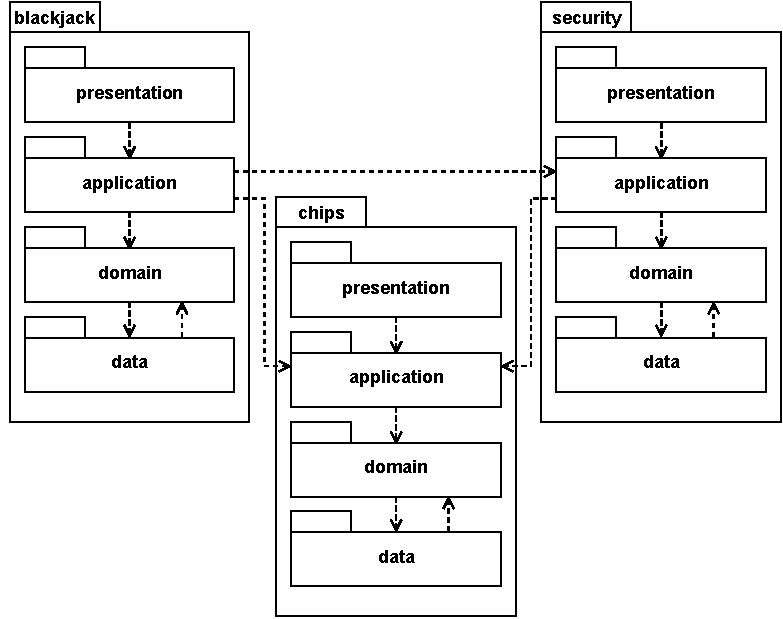
\includegraphics[width=.6\linewidth]{uml-casino-physical-layers}
    \caption{Components en layers kunnen met packages worden aangewezen binnen het casinoproject.}
    \label{fig:uml-casino-physical-layers}
\end{figure}

\subsubsection{Componenten}
Een component is een opzichzelfstaand onderdeel van een softwaresysteem
dat ziet op een bepaald deelgebied aan functionaliteit, bijvoorbeeld op een 
bepaald subdomein.

Het component bevat een aantal domeinobjecten. 
De communicatie wordt aangeboden via een service (ook: \textit{facade}). 
Deze service kan worden aangesproken door andere
services, maar ook door bijvoorbeeld een controller of een commando uit een commandline interface. 
De controller is bedoeld om HTTP-communicatie om te zetten naar Java code en vice versa. 
Andersom praat het component alleen met de buitenwereld, zoals een database, via een \textit{gateway}.

In ons project maken we gebruik van Spring om controllers te schrijven.
Deze controllers kunnen dan door Spring worden aangeroepen 
wanneer een bepaald web request moet worden afgehandeld.
Aan de andere kant maken we ook gebruik van Spring om te voorzien in 
de data-opslag aan de hand van repositories.
Repositories (\textit{gateways}) zijn bedoeld om door Spring 
te worden geïmplementeerd op basis van de benodigde opslagbehoeften.
In ons geval hebben we in \textit{application.properties} ingesteld dat het 
een PostgreSQL-database betreft.

\subsubsection{Lagen}
Een applicatie, of een deel ervan, is vaak opgedeeld in lagen die 
elk verantwoordelijk zijn voor een ander soort logica binnen het systeem.
Het afhandelen van gebruikersinteractie 
is bijvoorbeeld iets heel anders dan het uitdelen van kaarten in een
kaartspel of het opslaan van een speelronde.
Een gelaagde structuur helpt niet alleen met het terugvinden van
bepaalde klassen op basis van het soort logica dat het betreft. Bij een 
losgekoppeld ontwerp kunnen lagen of onderdelen ervan gemakkelijk uitgewisseld worden.

Gelaagde architecturen komen in verschillende soorten en maten. Sommige applicaties 
zijn eerst opgesplitst in componenten en vervolgens ingedeeld in lagen. Andere zijn 
eerst opgesplitst in lagen, waarin vervolgens losse componenten zijn te bespeuren.
Het aantal lagen kan variëren tussen de twee en vijf lagen. Dit hangt af 
van de verschillende soorten logica en de specifieke architecturele eisen
van de onderdelen binnen een project.

Deze packages corresponderen met de volgende soorten logica:
\begin{itemize}
    \item \emph{Presentation}: Presentatielogica. In het geval van een back-end API tref
    je hier alles aan dat hoort bij de technische vertaling van web requests naar Java-code. 
    Controllers (web request handlers) worden aangeroepen door het Spring framework 
    zodra een HTTP-request binnenkomt met een gedefinieerde route (HTTP-method + URL).
    \item \emph{Application}: Taakspecifieke logica. Hierin zitten applicatieservices (\emph{facades}) 
    die use cases omzetten naar domeinacties met behulp van infrastructuurabstracties. Een applicatieservice
    ziet vaak op één centraal domeinobject dat is opgebouwd uit of verwijst naar andere domeinobjecten.
    Door een applicatielaag in te richten kan dezelfde logica geboden worden onafhankelijk van de gebruikte 
    technologie in de presentatielaag: command line commando's, GUI's, web controllers of message handlers.
    \item \emph{Domain}: Domeinlogica. Domeinconcepten, business rules en entiteiten vind je vaak in lagen 
    met deze verantwoordelijkheid.
    \item \emph{Data}: Infrastructuurabstractie. Hierin zitten meestal interfaces of abstracte klassen die door
    infrastructuurklassen moeten worden ingevuld (\emph{gateways}). De daadwerkelijke infrastructuurlogica 
    wordt in het casinoproject ingevuld door het Spring framework. Hierover later meer.
\end{itemize}

\subsubsection{Kanttekening: Geen écht lagenmodel}
Het casinoproject is opgezet met de verschillende soorten logica in gedachten. 
Als je het lagenmodel echter strikt zou toepassen op Figuur~\ref{fig:uml-casino-physical-layers}, 
zie je een overtreding in de laatste twee lagen van elk component. 
Hier gaan we later in dit collegejaar op in (bij de cursus \textbf{Software Architecture}),
maar misschien wil je hier al wat meer over weten.

De datalaag bestaat weliswaar slechts uit interfaces die door 
Spring geïmplementeerd worden, maar ze zijn afhankelijk van objecten (entiteiten) die
gedefinieerd zijn in het domein. Logisch gezien zou je het project daarom 
eerder beschouwen als een drie-lagen-architectuur! De laatste laag zou dan 
conceptueel zowel domeinlogica als infrastructuurabstracties bevatten. 
Deze laag is dan fysiek (in onze code) opgedeeld in twee Java packages 
om de abstracte, stabiele kern (domein) te scheiden van de meer flexibele 
aansluiting met infrastructuur via interfaces (data). 
Het casino-project kent verder een flexible layered architecture: 
je mag lagen overslaan.
Zo mag je in de presentatielaag een domeinobject teruggeven,
zodat het in een HTTP-response kan worden opgenomen, en exceptions uit het domein 
afhandelen zodat een HTTP-response de juiste statuscode kan hebben.
Dit is in veel gelaagde architecturen niet het geval. In die architecturen 
heeft een laag alleen koppeling met de laag rechtstreeks eronder.
In ons project is dit niet nodig. Het scheelt een hoop extra code en we 
tolereren de extra koppeling.

\begin{figure}[H]
    \centering
    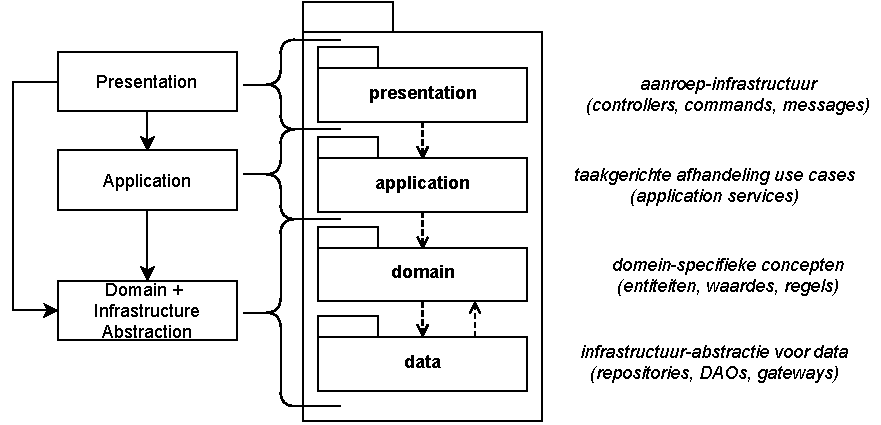
\includegraphics[width=.7\linewidth]{casino-layers}
    \caption{Het logisch en fysiek lagenmodel binnen het componenten van het casinoproject.}
    \label{fig:casino-layers}
\end{figure}

Als je de realisatie toch meer wil afstemmen op de laging, zou je de 
data-objecten en domein-objecten van elkaar splitsen en deze als losse objecten opnemen in de datalaag.
Daarvoor moet je dan daartussen een vertaalslag aanbieden. 
Als je daarnaast wil verbieden dat er lagen worden overgeslagen, 
zou je ook een vertaalslag kunnen toevoegen tussen domeinobjecten en presentatie-objecten.
Als alternatief zou je de infrastructuur-abstractie
(de repositories) kunnen opnemen in het domein en dat \textit{data} package verwijderen.
In ons project passen we deze regels echter niet zo strikt toe:
we accepteren een lichte koppeling op het framework en op ons domein.

\subsubsection{Subsystems}
Een laag kan nog verder worden opgebroken in subsystems (of \textit{deelsystemen}).
Dit zijn algemene packages die zijn bedoeld om een reeks objecten samen te verpakken.

\subsection{Voorbeeld: Structuur binnen het chips-component}
Elk component is in lagen opgedeeld. In het chips-component ziet 
dat eruit zoals in Figuur~\ref{fig:chips-layers}.

\begin{figure}[H]
    \centering
    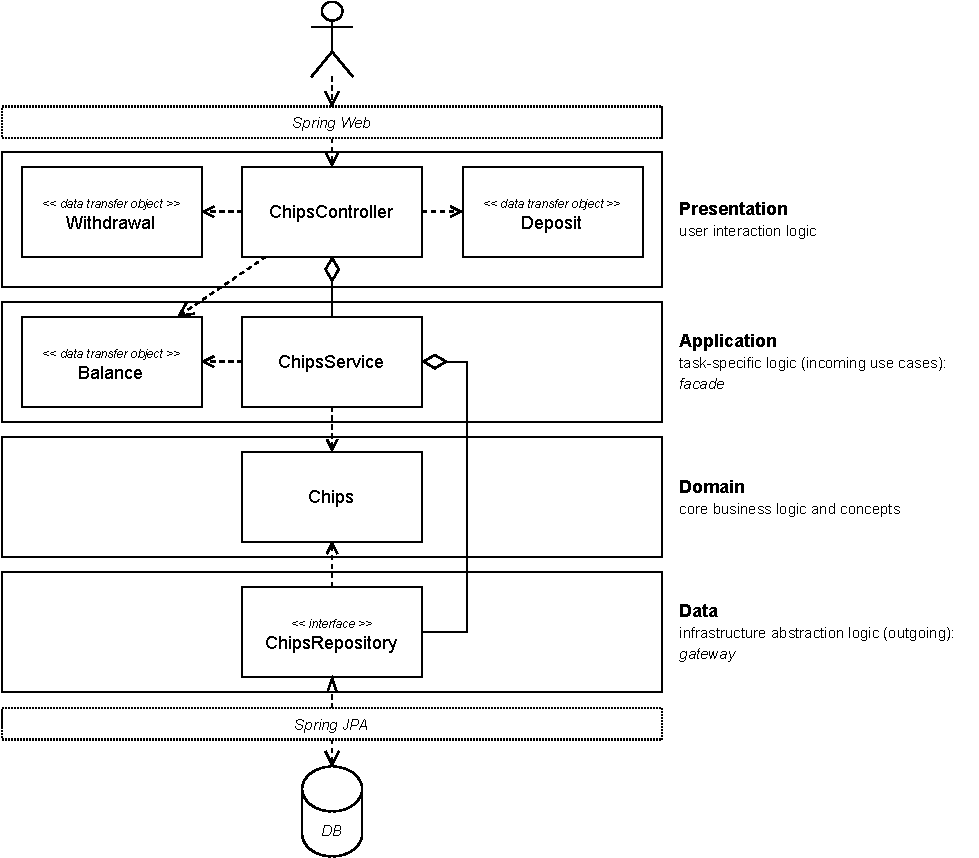
\includegraphics[width=0.8\linewidth]{chips-layers}
    \caption{De semi-gelaagde structuur binnen het chips-component.}
    \label{fig:chips-layers}
\end{figure}

Probeer voor jezelf de volgende vragen te beantwoorden, eventueel door naar de code te kijken.
Welke klasse is verantwoordelijk voor de vertaling van HTTP-verkeer naar Java en andersom?
In welke klassen zal je de use cases van dit component terugzien?
In welke methode wordt het aantal chips verminderd bij een afschrijving?
Hoe denk je dat de opslag geregeld is?
Stel een ander component binnen ons systeem wil Chips opnemen voor een user, welke klasse wordt dan 
eerst aangesproken?

Je mag dit met docenten en medestudenten overleggen, 
maar het antwoord op deze vragen zal naar verloop van tijd duidelijker worden.

\newpage
\subsection{Voorbeeld: Use cases van het chips-component}
Het chips-component biedt al een aantal use cases aan binnen ons systeem.
Deze zijn opgesomd in de ChipsService en laten zich gemakkelijk in een 
use case diagram vatten, zie: Figuur~\ref{fig:chips-use-cases}.
Kijk in de code of je dit kunt herkennen!

\begin{figure}[H]
    \centering
    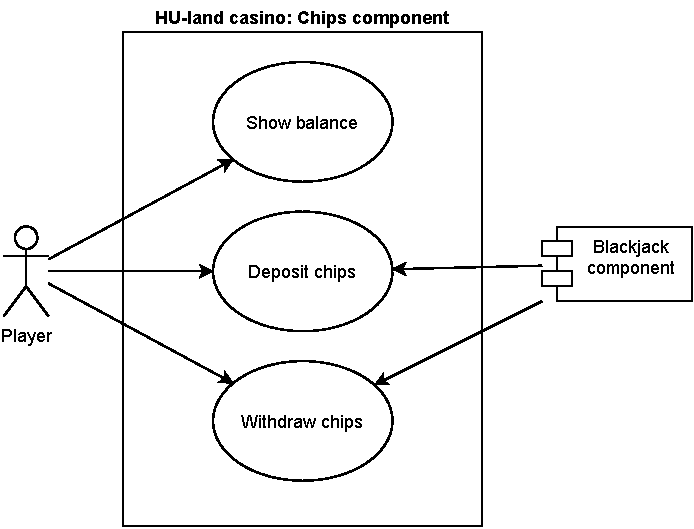
\includegraphics[height=0.4\linewidth]{chips-use-cases}
    \caption{De use cases van het chips-component}
    \label{fig:chips-use-cases}
\end{figure}

Zoals je ziet, willen we onze blackjack-component straks 
ook gebruik laten maken van de de chips-component!

\newpage
\subsection{Applicatieflow}
Hoe loopt de flow binnen de de lagen in een component? 
Laten we daarvoor een blik werpen 
op de \emph{deposit use case} van het Chips-component.
Zie Figuur~\ref{fig:chips-sequence-diagram}.

\begin{figure}[H]
    \centering
    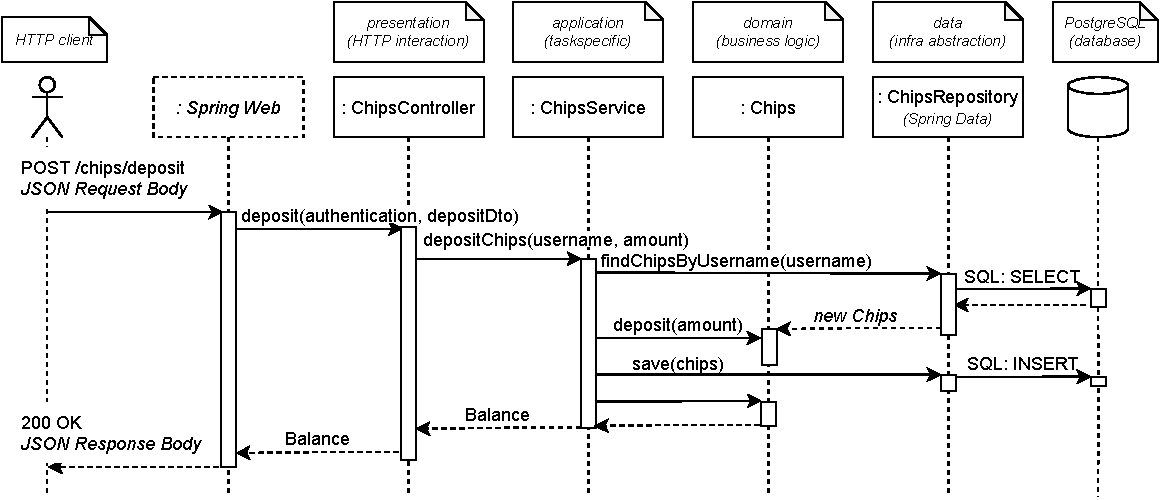
\includegraphics[width=\linewidth]{chips-sequence-diagram}
    \caption{De flow voor de deposit use case van het Chips-component}
    \label{fig:chips-sequence-diagram}
\end{figure}

Kijk ook in de code of je dit kunt herkennen!
Allereerst moet een HTTP-client een POST-verzoek doen naar 
\texttt{/chips/deposit}. We willen namelijk een overmaking toevoegen
aan de chips resource voor de huidige gebruiker. In dat POST-verzoek 
wordt de huidige gebruiker meegegeven via een JWT-token in de Authorization header
als deze is ingelogd. 

Vervolgens zet Spring Web dit verzoek om naar de bijbehorende 
controlleractie op de \emph{ChipsController} in de presentatielaag, met de
nodige informatie over de gebruiker (\emph{Authentication}) en de data die 
in de HTTP JSON Request Body zit (het \emph{Deposit} data transfer object).
De controller haalt de nodige data uit deze objecten en zet dit om naar 
een aanroep op de \emph{ChipsService} in de applicatielaag. 
Deze ChipsService bevat allerlei methoden die de use cases van 
het Chips-component vertegenwoordigen.
De service roept de \emph{ChipsRepository} aan uit de datalaag om de hoeveelheid
\emph{Chips} op te vragen voor de betreffende \emph{User} (op basis van de username). 
Vervolgens roept de service de \emph{deposit}-methode aan op de Chips om het aantal chips te verhogen met de 
gekozen hoeveelheid en wordt het \emph{Chips} object weer opgeslagen in de \emph{ChipsRepository}.
Ten slotte geeft de service een \emph{Balance} terug door de benodigde data uit het 
\emph{Chips}-object te halen en dit in een nieuw \emph{Balance}-object te stoppen.
De controller geeft ook deze \emph{Balance} terug aan Spring Web, waarop deze de 
\emph{Balance} omzet naar een HTTP JSON Response Body aan de hand van diens getters.

Voor het blackjack-component zou het ideaal zijn als wij ook één centraal object hebben 
om op te halen, domeinacties op uit te voeren en weer weg te schrijven. Het aan elkaar 
knopen daarvan kan gebeuren in use cases aangeboden in een BlackjackService!